\documentclass[one column]{report}
\usepackage[utf8]{inputenc}

\usepackage{amsmath,amsthm,amssymb}

\usepackage{subcaption}
\usepackage{graphicx}

\usepackage{comment}

\usepackage{bm}
\renewcommand{\b}[1]{\bm{#1}}
\newcommand{\tr}{\text{ tr }}
\newcommand{\cov}[2]{\text{cov}(#1,#2)}
\newcommand{\corr}[2]{\text{corr}(#1,#2)}
\newcommand{\mean}[1]{\overline{\b{#1}}}
\usepackage{diagbox}
\newcommand{\abs}[1]{
  \left|
    #1
  \right|}
\newcommand{\rank}[1]{\text{rank #1}}
\newcommand{\diag}{\text{diag }}

\usepackage{biblatex}
\bibliography{ref}

\graphicspath{{./images/}}

\usepackage{listings}


\usepackage{color}

\definecolor{gray}{rgb}{0.5,0.5,0.5}
\definecolor{orange}{rgb}{0.8,0,0}

\lstdefinestyle{matlab}{
  belowcaptionskip=1\baselineskip,
  breaklines=true,
  frame=L,
  xleftmargin=\parindent,
  language=octave,
  showstringspaces=false,
  basicstyle=\footnotesize\ttfamily,
  keywordstyle=\bfseries\color{green},
  commentstyle=\color{gray},
  identifierstyle=\color{blue},
  stringstyle=\color{orange},
}
\lstdefinestyle{R}{
  belowcaptionskip=1\baselineskip,
  breaklines=true,
  frame=L,
  xleftmargin=\parindent,
  language=R,
  showstringspaces=false,
  basicstyle=\footnotesize\ttfamily,
  keywordstyle=\bfseries\color{green},
  commentstyle=\color{gray},
  identifierstyle=\color{blue},
  stringstyle=\color{orange},
}

\def\listingsfont{\ttfamily} 
\def\listingsfontinline{\ttfamily}

\title{TAMS39 - Examination exercises}
\author{Anton Karlsson\\antka388\\931217-7117}
\date{}
\begin{document}
\maketitle

\section*{Exercise 1}

\subsection*{(a)}
\label{sec:a}

Let $H_0: \b \mu_{\rm  male} = \b \mu_{\rm female}$ against $H_{1}: \b \mu_{\rm
  male} \neq \b \mu_{\rm female}$.
We get the test statistic $T^{2}$ which is given by
\begin{equation*}
  T^{2} = n(\mean X - \b \mu_{\rm male})^{T} S^{-1}(\mean X - \b \mu_{\rm male}),
\end{equation*}
where $\b S = \frac{1}{n-1}(\b X - \b 1\mean X^{T})(\b X - \b 1\mean
X^{T})^{T}$, $\b \mu_{\rm male} = (190, 275)^{T}$, and $n$ is the size
of the population. If $p$ is the dimension of the population, then 
\begin{equation*}
  \frac{n-p}{(n-1)p}T^{2} \sim F(p,n-p+1).
\end{equation*}
A test given by rejecting $H_{0}: T^{2} \geq \frac{(n-1)p}{n-p}F_{p,
  n-p}(1 -\alpha) = c_{\alpha}$, where $\alpha = 0.05$. We get that
$c_{\alpha} \approx 6.58$ and $T^{2} \approx 5.54
$, thus we cannot reject $H_{0}$.


\subsection*{(b)}
\label{sec:b}

The confidence region is given my all $\b \mu$ such that
\begin{equation*}
  n(\mean X - \b \mu)^{T}\b S^{-1}(\mean X - \b \mu) \leq \frac{(n-1)p}{n-p}F_{p,
  n-p}(1 -\alpha) = c_{\alpha}.
\end{equation*}
The result is displayed in Figure \ref{fig:ex1-ellipse}.
\begin{figure}[h]
  \centering
  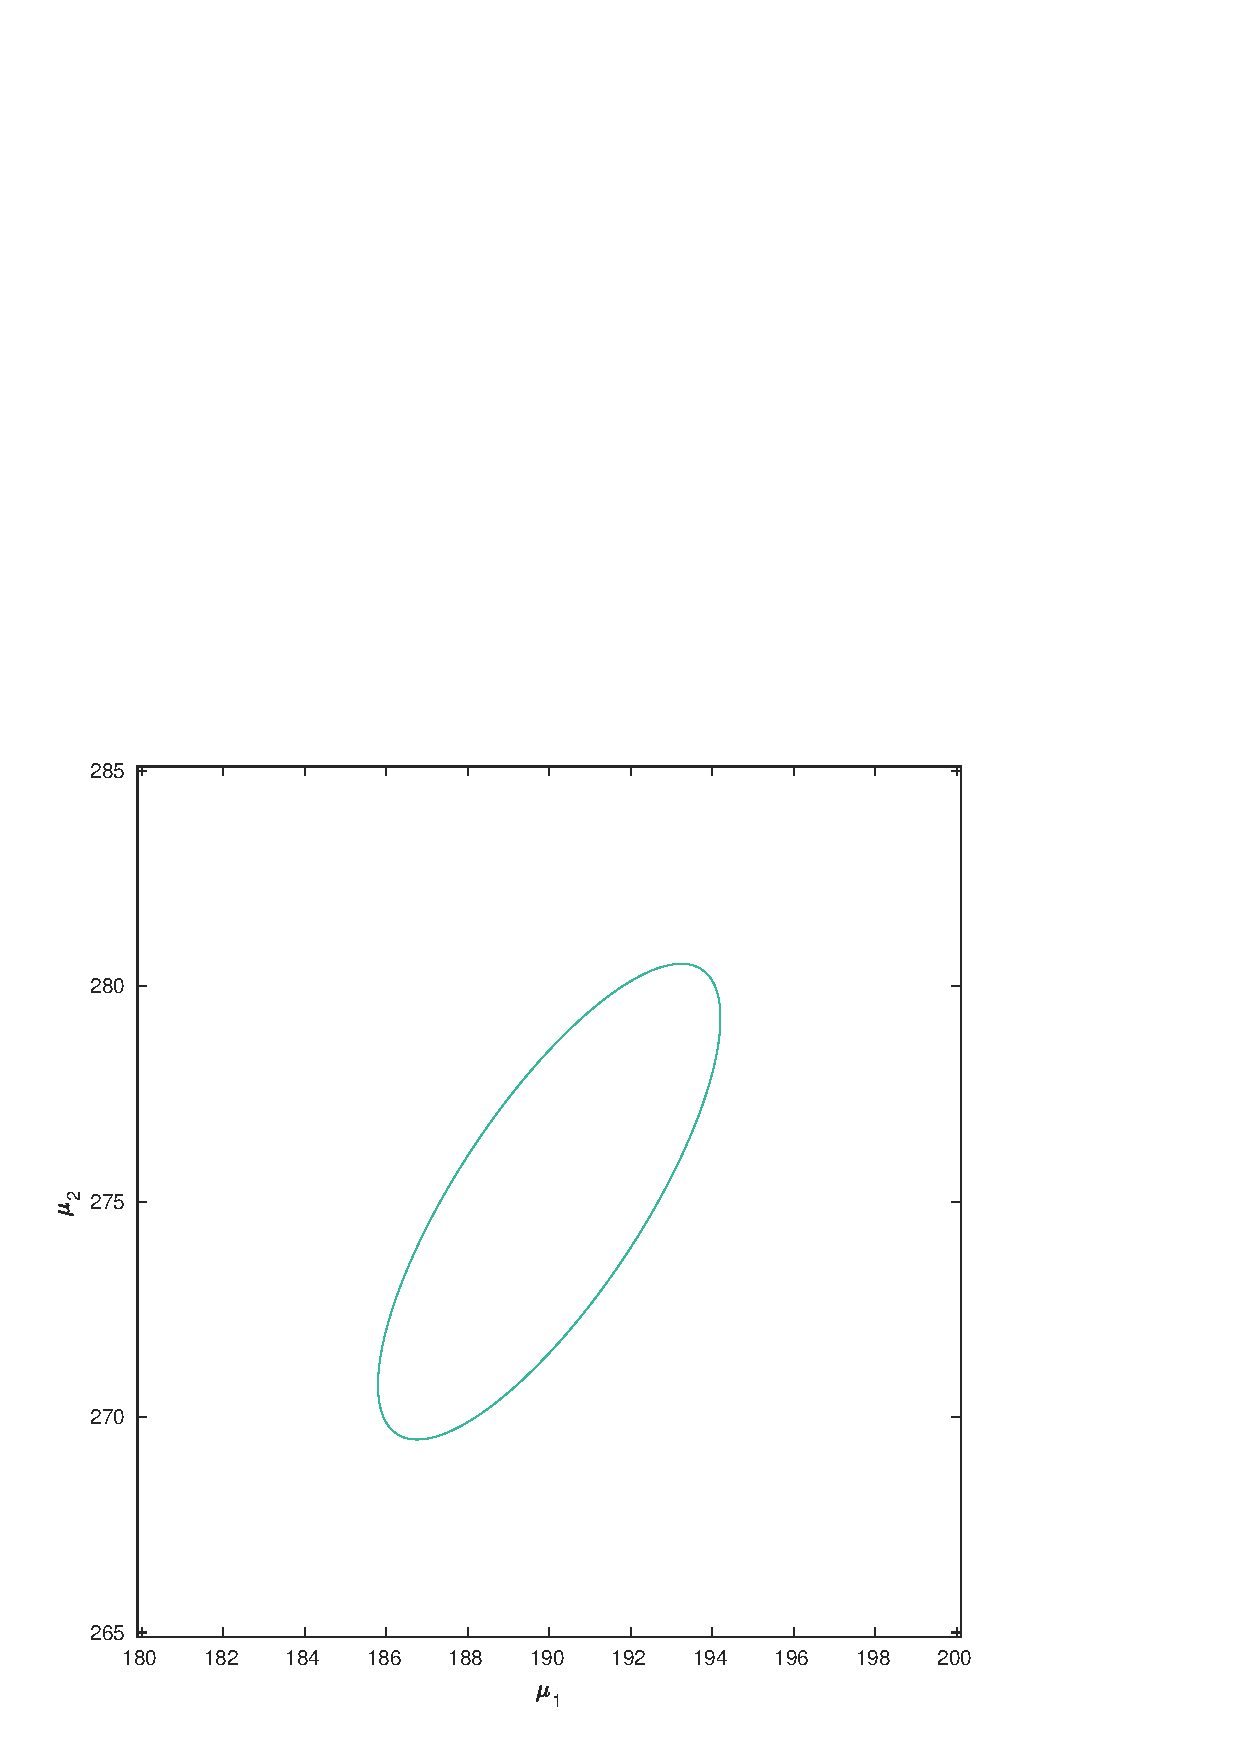
\includegraphics[width=5cm]{ellipse-ex1}
  \caption{The confidence ellipse around ${\bf \mu}$.}
  \label{fig:ex1-ellipse}
\end{figure}

\subsection*{(c)}
\label{sec:c}

From Result 5.3 in \cite[p. 225]{book} we get that simultaneously
confidence interval for $\b a' \b \mu$ is  given by
\begin{equation*}
  \b a^{T} \mean X - \sqrt{\frac{(n-1)p}{n(n-p)}F_{p,
  n-p}(1 -\alpha) \b a^{T}\b S\b a} \leq \b a^{T} \b \mu \leq 
\b a^{T} \mean X + \sqrt{\frac{(n-1)p}{n(n-p)}F_{p,
  n-p}(1 -\alpha) \b a^{T}\b S\b a} .
\end{equation*}
We get that for $\b a = (1, 0)^{T}$, which represents $\mu_{1}$, and for
$\b a = (0,1)^{T}$, which represents $\mu_{1}$, the confidence
intervals are
\begin{equation*}
  \begin{pmatrix}
    185.80 &194.20 
  \end{pmatrix},\quad \text{and} \quad
  \begin{pmatrix}
    269.48 &280.52  
  \end{pmatrix},
\end{equation*}
respectively.\\
\\
The Bonferroni intervals are given by 
\begin{equation*}
  \overline{x}_{i} \pm t_{n-1}(1 - \alpha/(2m) )\sqrt{\frac{s_{ii}}{n}},
\quad i = 1,2,
\end{equation*}
where $m= 2$ is the number of intervals. The intervals for
$\mu_{1}$ and $\mu_{2}$ are
\begin{equation*}
  \begin{pmatrix}
    186.20 &193.80 
  \end{pmatrix}, \quad \text{and}\quad
  \begin{pmatrix}
    270.00 &280.00 
  \end{pmatrix},
\end{equation*}
respectively.\\
\\
One advantage that the $T^{2}$-intervals have over the corresponding
Bonfferoni intervals is that the
Bonfferoni intervals are given by the inequaltiy
\begin{equation*}
  P\left(\text{the interval }\overline{x}_{i} \pm t_{n-1}(1 - \alpha/(2m)
  )\sqrt{\frac{s_{ii}}{n}}\text{ contains }\mu_{i},
\quad \text{for }i = 1,2,\right) \leq 1 - \alpha,
\end{equation*}
which the $T^{2}$-intervals do  not have; they have an equality
instead, meaning that the $T^{2}$-intervals can be more accurate than
the Bonfferoni intervals. 
%%% Local Variables:
%%% mode: latex
%%% TeX-master: "examination"
%%% End:

\section*{Exercise 2}
\label{sec:exercise-2}

\subsection*{(a)}
\label{sec:a-1}

The scatter plot can be found in Figure \ref{fig:ex2-scatter} the outlier can be
clearly be seen at $x_1 = 284$.
\begin{figure}[h]
  \centering
  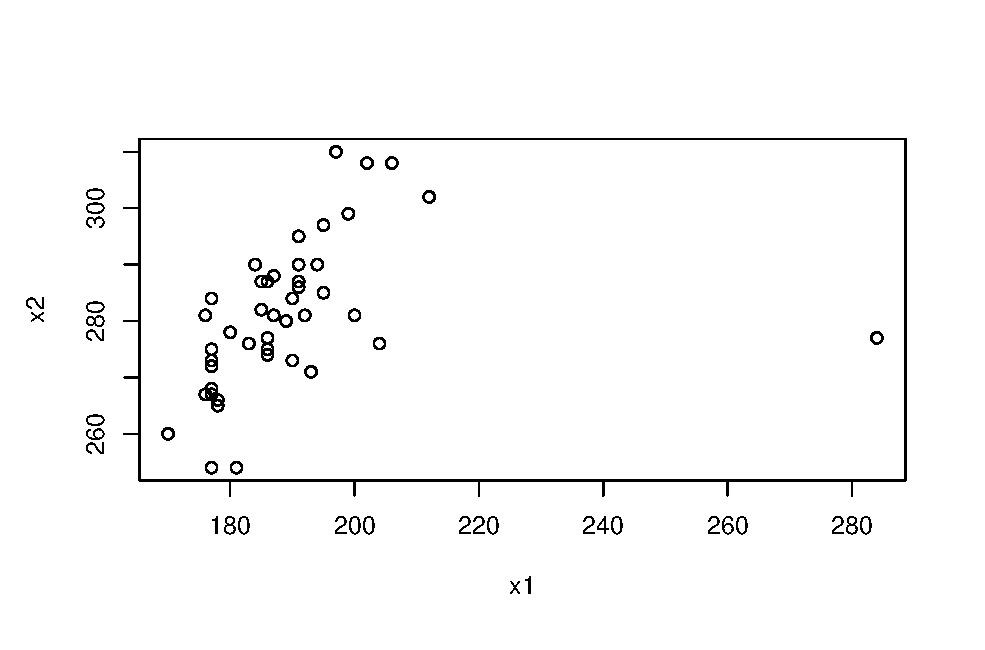
\includegraphics[width=5cm]{ex2-scatterplot}
  \caption{Scatter plot of the tail length and the wing span for male
    hook-billed kites.}
  \label{fig:ex2-scatter}
\end{figure}

\subsection*{(b)}
\label{sec:b-1}

We remove the sample with $x^{\rm male}_{1} = 284$.
Let $H_{0}: \b S_{\rm male} = \b S_{\rm female}$ versus $A \neq
H$. For this test we can use Box's test for equality of covariance
matrices, in which we reject $H_{0}$ if 
\begin{equation*}\label{eq:boxcorrection}
  (1 - u)
  \left(
    \left[
      \sum_{i=1}^{2}(n_{i} - 1)
    \right]
    \ln \abs{\b S_{\rm pooled}} - \sum_{i=1}^{2}(n_{i}-1) \ln \abs{\b S_{i}}
  \right) > \chi^{2}_{p(p+1)(g-1)/2}(1-\alpha),
\end{equation*}
where $p=2$ is the dimension of the populations, $g = 2$ is the
number of groups in the experiment, and
\begin{equation*}
  u = 
  \left[
    \sum_{i=1}^{2}\frac{1}{n_{i}-1} - \frac{1}{\sum_{i=1}^{2}(n_{i}-1)}
  \right]
  \left[
    \frac{2p^{2} + 3p - 1}{6(p+1)(g-1)}
  \right].
\end{equation*}
We represent the male population with $i=1$ and the female by
$i=2$. The covariance matrices $\b S_{i}$ is the sample mean for $i =
1,2$, and the pooled matrix, $\b S_{\rm pooled}$, is given by 
\begin{equation*}
  \b S_{\rm pooled}=  \frac{1}{\sum_{i=1}^{2}(n_{1} -
    1)}\sum_{i=1}^{2}(n_{i}-1)\b S_{i}  .
\end{equation*}
We get that 
\begin{equation*}
    (1 - u)
  \left(
    \left[
      \sum_{i=1}^{2}(n_{i} - 1)
    \right]
    \ln \abs{\b S_{\rm pooled}} - \sum_{i=1}^{2}[(n_{i}-1) \ln \abs{\b S_{i}}]
  \right) \approx 1.0431
\end{equation*}
and
\begin{equation*}
  \chi^{2}_{p(p+1)(g-1)/2}(1-\alpha) \approx 7.8147 , \quad \alpha =0.05.
\end{equation*}
Hence we should not reject $H_{0}$, the matrices can be pooled. On the
other hand, if we  instead change the outlier earlier to
$x_{1}^{\rm male} = 184$, we get that 
\begin{equation*}
    (1 - u)
  \left(
    \left[
      \sum_{i=1}^{2}(n_{i} - 1)
    \right]
    \ln \abs{\b S_{\rm pooled}} - \sum_{i=1}^{2}[(n_{i}-1) \ln \abs{\b S_{i}}]
  \right) \approx 1.2223,
\end{equation*}
and the same conclusion holds.
\subsection*{(c)}
\label{sec:c-1}
We remove the outlier.
 Using Result 6.2 in \cite[p. 286]{book} we can use the $T^{2}$ test
 where we accept $H_{0}:\b \mu_{\rm male} = \b \mu_{\rm female}$ versus
 $H_{1}:\b \mu_{\rm male} \neq \b \mu_{\rm female}$ if 
\begin{equation*}
T^{2} = \b Y^{T}
\left[
  \left(
    \frac{1}{n_{\rm male}} + \frac{1}{n_{\rm female}}
  \right)
  \b S_{\rm pooled}
\right]^{-1} \b Y
\leq \frac{(n-2)p}{n-1+p}F_{p, n-1+p}(1-\alpha) =:c^{2}_{\alpha},
\end{equation*}
with a confidence level of $1-\alpha$, where $\b Y = \b X_{\rm male}- \b
X_{\rm female} - (\mean X_{\rm male}- \mean X_{\rm female} )$ and $n$ is the total number of samples. From the given data, we get that
 $T^{2}\approx 24.96 $
and $c^{2}_{\alpha} \approx 6.28$, thus we reject $H_{0}$. \\
\\
If we instead change the outlier to 184, we get $T^{2} \approx 25.66$ and
$c_{\alpha}^{2} \approx  6.27$, so we get the same conclusion as when
we removed the outlier; $H_{0}$ is rejected.
\subsection*{(d)}
 From the remark found in \cite[p. 289]{book}, the linear combination
 $\b a^{T} (\mean x_{\rm male} - \mean x_{\rm female})$ with $\b a
 \propto \b S_{\rm pooled}^{-1}(\mean x_{\rm male} - \mean x_{\rm
   female}) =
 \begin{pmatrix}
   -0.16 &0.09
 \end{pmatrix}^{T}
$ is most responsible for rejecting $H_{0}$ in Exercise (c). 
\subsection*{(e)}
\label{sec:e}

The confidence region if given by the equation
\begin{align}
  \label{eq:ex2-conf-region}
 (\mean x_{\rm male}  - \mean x_{\rm female} - \b \mu)^{T}
\left[
  \left(
    \frac{1}{n_{\rm male}} + \frac{1}{n_{\rm female}}
  \right)
  \b S_{\rm pooled}
\right]^{-1} (\mean x_{\rm male}  - \mean x_{\rm female} - \b \mu) \nonumber
\\
\leq \frac{(n-2)p}{n-1+p}F_{p, n-1+p}(1-\alpha) =:c^{2}_{\alpha}
\end{align}
where for $\mu = (\mu_1, \mu_2)$, and $\alpha = 0.05$. The confidence
ellipse is represented in Figure \ref{fig:ex2fig}.

\begin{figure}[h]
  \centering
  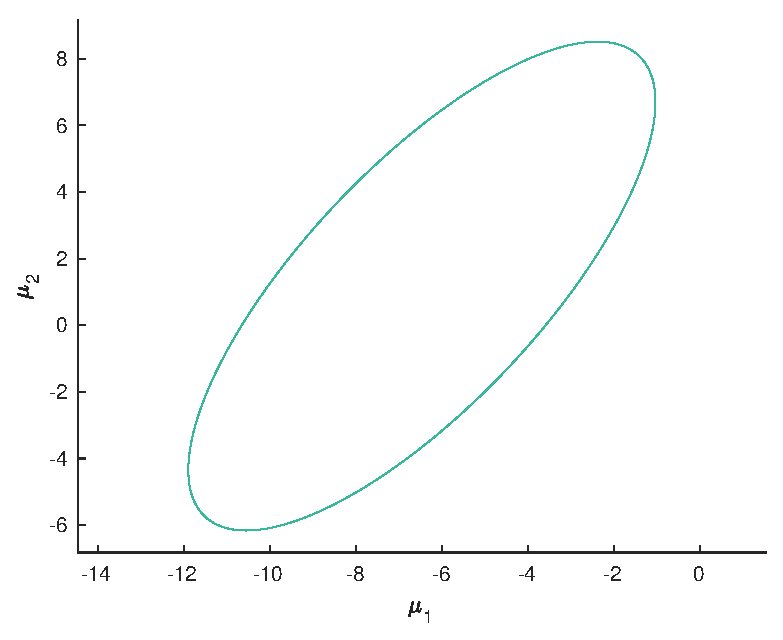
\includegraphics[width=10cm]{ex2fig}
  \caption{The confidence region of the difference
    $\b \mu_{\rm male} - \b \mu_{\rm female}$ with confidence 95\%. }
  \label{fig:ex2fig}
\end{figure}
The simultaneous confidence interval are $\b \mu = \b \mu_{\rm male}- \b
\mu_{\rm female}$ then we get that the confidence region for $\mu_{1}$
is given by 
\begin{equation*}
  \begin{pmatrix}
   -11.90 &-1.03  
  \end{pmatrix}
\end{equation*}
and, for $\mu_{2}$, 
\begin{equation*}
  \begin{pmatrix}
   -6.16 &8.52  
  \end{pmatrix}.
\end{equation*}
The confidence intervals ''frames'' the confidence region, as is shown
in Figure \ref{fig:ex2_sim_intervals}. 
\begin{figure}[h]
  \centering
  \includegraphics[width=10cm]{ex2fig_with_sim_intervals}
  \caption{Confidence region with and the simultaneous $T^{2}$-intervals plotted. }
  \label{fig:ex2_sim_intervals}
\end{figure}
\subsection*{(f)}
\label{sec:f}
There is evidence for that female birds have longer tails. However,
there is no significant difference between the genders when it comes to
the length of their wingspan. 


%%% Local Variables:
%%% mode: latex
%%% TeX-master: "examination"
%%% End:


\section*{Exercise 3}
\label{sec:exercise-3}

\subsection*{(a)}
\label{sec:a-2}
The plot of the profiles are presented in figure
\ref{fig:ex3-profiles}.
\begin{figure}[h]
  \centering
  \includegraphics[width=8.5cm]{ex3-profiles}
  \caption{The profiles for the Psychmotor scores given different
    radiation treatment.}
  \label{fig:ex3-profiles}
\end{figure}

\subsection*{(b)}
\label{sec:b-2}


Since we have more than tho profiles we wich to test, we have to use
the more general approach. Set up the variables as descibed in Lectrure
6. We can test if the profiles are parallel using
\begin{equation*}
  \lambda_{H_1} = \frac{\det CVC^T}{\det( CVC^T  + CHC^T),}
\end{equation*}
and createing the test variables
\begin{equation*}
  test = -\left(n - \frac 12(k + p -1)\right) \ln \Lambda_{H_1},
\end{equation*}
which is $\chi^2((p-1)(k-1))$. We reject $H_1$ if test variable is
smaller then the critical point, 
\begin{equation*}
  c = \chi^2 _{0.95} ((p-1)(k-1)).
\end{equation*}
From matlab we get
\begin{equation*}
  test = -4.0443,
\end{equation*}
and
\begin{equation*}
    c = 12.5916.
\end{equation*}
Since we $test < c$, we can not reject $H_1$, the profiles are parallel.


\subsection*{(c)}
\label{sec:c-2}

Since, the profiles are parallel, we can set up a test for checking if
the profiles are on the same level. This can be done by using the test
\begin{equation*}
  \lambda_{H_2 | H_1} = \frac{\det(CVC^T + CHC^T)}{\det(CVC^T)}\frac{\det(V)}{\det(V+H)},
\end{equation*}
and creating the test variable 
\begin{equation*}
  F = \left(\frac{n-k - p +1}{k - 1}\right)\frac{1 - \lambda_{H_2 |H_1}}{\lambda_{H_2 | H_1}},
\end{equation*}
which we compare to the critical value
\begin{equation*}
  c = F_{0.95} (k-1, n - k - p +1).
\end{equation*}
We get
\begin{equation*}
  -10.8296 = F < c = 2.8451,
\end{equation*}
we can not reject $H_2 | H_1$, the profiles are on the same level.

\subsection*{(d)}
\label{sec:d-1}

Here, we use the test variables 
\begin{equation*}
  \lambda_{H_3 | H_1} = \frac{1}{1 + n \bar{\bf x}^T C^T (CVC^T +
    CHC^T)^-1C*\bar{\bf x}},
\end{equation*}
and create the test variable
\begin{equation*}
  test = \frac{n - p +1}{p - 1}\lambda_{H_3 |H_1},
\end{equation*}
which we compare to 
\begin{equation*}
  c = F_{0.95}(p-1, n-p+1).
\end{equation*}
We get
\begin{equation*}
  7.9361 = test > c = 3.2145.
\end{equation*}
So we get that we have to reject $H_3 | H_1$, the profiles are not
flat.

\section*{\texttt{matlab} code}
\label{sec:textttmatlab-code}

\lstinputlisting[style=matlab]{../ex3.m}
%%% Local Variables:
%%% mode: latex
%%% TeX-master: "examination"
%%% End:


\section*{Exercise 4}
\label{sec:exercise-4}

\subsection*{(a)}
\label{sec:a-3}

We can check if the matrices can be pooled by using the test variable
\begin{equation*}
  \lambda^* = \frac{\Pi \det(V_i ^{f_i/2})}{\det(V^{f/2})}
  \frac{f^{pf/2}}{\Pi f_i ^{pfi/2}}
\end{equation*}
and using the Box correction, we get
\begin{equation*}
  -2  \frac{m}{f} \ln \lambda^* = 49.2750,
\end{equation*}
which we comapre against the critical value
\begin{equation*}
  c = \chi^2_{0.95}(f) = 58.1240,
\end{equation*}
hence the covariance matrices can be pooled into one matrix.

\subsection*{(b)}
\label{sec:b-3}

We could calculate the linear seprators, $ l_i^T x_0 + c_i$, where
we obtain
\begin{align*}
l_1^T x_0 + c_1 &= (-0.57, 1.80, 1.01, 6.33, 18.94, 0.33)x_0 + -703.95 \\ 
l_2^T x_0 + c_2 &= (-0.14, 1.31, 1.48, 5.15, 18.31, 0.04)x_0 + -554.06 \\ 
l_3^T x_0 + c_3 &= (-1.08, 1.89, 3.03, 5.69, 15.11, 0.51)x_0 + -618.43,
\end{align*}
In which we can conclude that ${\bf x_0}$ belongs to  $\pi_i$ if $
  l_i^T x_0 + c_i = \max_i \left(   l_i^T x_0 + c_i\right)
$

\subsection*{(C)}
\label{sec:c-3}

Since we have unkwn mean and variance, we use the approximation 
\begin{align*}
  e_1 &= \phi(\Delta) \frac{\Delta^2 + 12(p-1)}{16\Delta} \\
  e_2 &=  \phi(\Delta)\frac{\Delta^2 - 4(p-1)}{16\Delta},
\end{align*}
where $\Delta$,  $a_1$ and $a_2$  are defined as in the lectures.
Using the pooled matrix $S_p$ for all three populations, we got the
probablity of classifying wrongly into $\pi_1$ to be
\begin{equation*}
  e_1 \approx 0.0019
\end{equation*},
and for $\pi_2$ to be
\begin{equation*}
  e_2  \approx 0.0019.
\end{equation*}
\subsection*{Code}
\label{sec:code}



\lstinputlisting[style=matlab]{./../ex4.m}
%%% Local Variables:
%%% mode: latex
%%% TeX-master: "examination"
%%% End:


\section*{Exercise 5}
\label{sec:exercise5}

\subsection*{(a)}
\label{sec:a-4}

The dot diagrams are shown in Figure \ref{fig:ex5-marginalplots}. 

\begin{figure}[h]
  \centering
  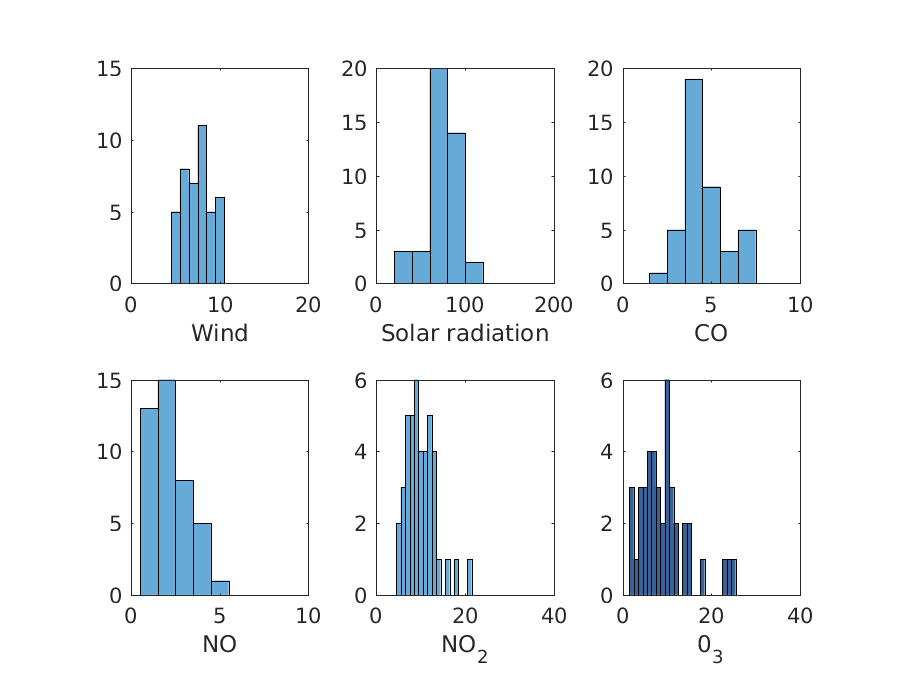
\includegraphics[width=13cm]{ex5-marginalplots}
  \caption{The marginal dot diagrams for all variables}
  \label{fig:ex5-marginalplots}
\end{figure}

\subsection*{(b)}
\label{sec:b-4}

The sample mean is given as
\begin{equation*}
  \bar{x} =
  \begin{pmatrix}
    7.50 & 73.86 & 4.55 & 2.19 & 10.05 & 9.40 & 3.10 
  \end{pmatrix}^T
\end{equation*}
and
\begin{equation*}
  S =
  \begin{pmatrix}
    2.50 & -2.78 & -0.38 & -0.46 & -0.59 & -2.23 & 0.17 \\ 
    -2.78 & 300.52 & 3.91 & -1.39 & 6.76 & 30.79 & 0.62 \\ 
    -0.38 & 3.91 & 1.52 & 0.67 & 2.31 & 2.82 & 0.14 \\ 
    -0.46 & -1.39 & 0.67 & 1.18 & 1.09 & -0.81 & 0.18 \\ 
    -0.59 & 6.76 & 2.31 & 1.09 & 11.36 & 3.13 & 1.04 \\ 
    -2.23 & 30.79 & 2.82 & -0.81 & 3.13 & 30.98 & 0.59 \\ 
    0.17 & 0.62 & 0.14 & 0.18 & 1.04 & 0.59 & 0.48 \\ 
  \end{pmatrix}
\end{equation*}

\subsection*{(c)}
\label{sec:c-4}

The model used was
\begin{equation*}
  y_1 = \beta_0 + \beta_1 x_1 + \beta_2 x_2 + \epsilon,
\end{equation*}
where $\hat{\beta} = (10.1145,\   -0.2113,\    0.0205)$. From here we
can calculate the residual:
\begin{equation*}
  \text{SS}_{\rm E} = 455.1356.
\end{equation*}

Further, we got the following confidence interval with confidence level of 95
\%: $(7.59, 11.71)$. 

\subsection*{(d)}

Here, we propose the linear model
\begin{equation*}
  \begin{pmatrix}
    y_1 \\ y_2
  \end{pmatrix} = 
  BX + E,
\end{equation*}
where 
\begin{equation*}
  X =
  \begin{pmatrix}
    {\bf 1_n} & x_2 & x_2
  \end{pmatrix}.
\end{equation*}
We found that
\begin{equation*}
  B =
  \begin{pmatrix}
    10.11 & -0.21 \\ 
    0.02 & 8.28 \\ 
    -0.79 & 0.10 
  \end{pmatrix}.
\end{equation*}

The confidence region for $x_1 = 10$ and $x_2 = 80$ is shown in Figure
\ref{fig:ex5-ellipse}
\begin{figure}[h]
  \centering
  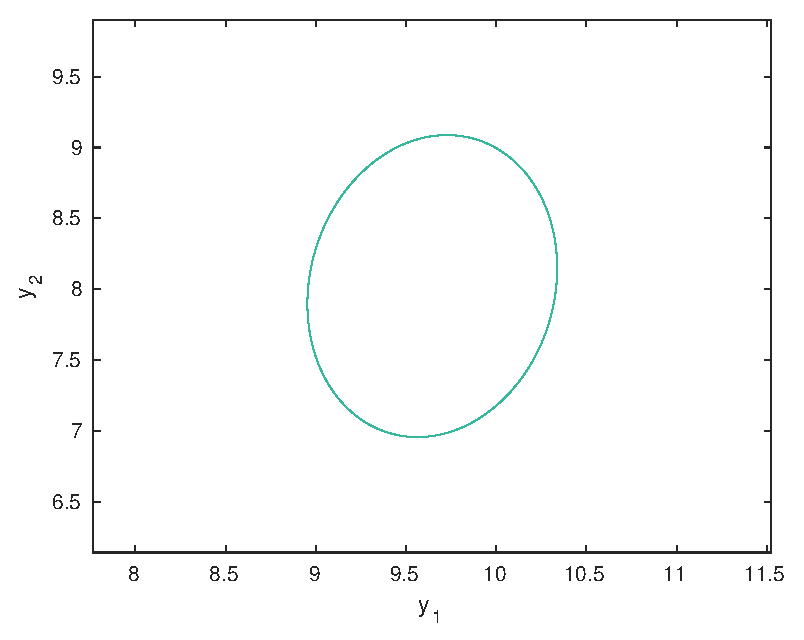
\includegraphics[width=7cm]{ex5-ellipse}
  \caption{The confidence region for $x_1 = 10$ and $x_2 = 80$. }
  \label{fig:ex5-ellipse}
\end{figure}

We can see that the ellispe is covered by 
the confidence interval in Exercise~(c), on the $y_1$ axis.

%%% Local Variables:
%%% mode: latex
%%% TeX-master: "examination"
%%% End:

\section*{Exercise 6}
\label{sec:exercise-6}

\subsection*{(a)}
\label{sec:a-5}


The following linear model was designed
\begin{equation*}
  \b Y = \b{XB} + \b E,
\end{equation*}
where $\b Y$ is the out parameters, $\b X = (\b 1_n, \b x_1, \b x_2)$
is the design matrix, and $\b B:(3 \times 4) $ contained the unknown parameters which
was estimated using linear regression as
\begin{equation*}
  \b\hat B =
  \begin{pmatrix}
    -94.60 &-228.67 &-258.80 &-246.05 &-232.96 \\ 
    19.27 &43.65 &48.99 &47.33 &45.10 \\ 
    -24.68 &-20.59 &3.32 &5.22 &8.24 
  \end{pmatrix}.
\end{equation*}

\subsection*{(b)}
The sample correlation matrix was 
\begin{equation*}
  \b R =
  \begin{pmatrix}
    1.00 &0.86 &0.71 &0.64 &0.65 &0.81 &-0.09 \\ 
    0.86 &1.00 &0.91 &0.89 &0.90 &0.95 &0.10 \\ 
    0.71 &0.91 &1.00 &0.98 &0.98 &0.92 &0.22 \\ 
    0.64 &0.89 &0.98 &1.00 &1.00 &0.90 &0.22 \\ 
    0.65 &0.90 &0.98 &1.00 &1.00 &0.90 &0.24 \\ 
    0.81 &0.95 &0.92 &0.90 &0.90 &1.00 &0.22 \\ 
    -0.09 &0.10 &0.22 &0.22 &0.24 &0.22 &1.00  
  \end{pmatrix}.
\end{equation*}
was isWhat is interesting is that the time steps that are close to each other
correlates more than those times further apart. We can even note that
the first and last time steps have negative correlation and is almost 0.

\subsection*{(c)}
\label{sec:c-5}

The average weight is governed by the last row in $\b B$, $\b B_{2}$, so therefore we
want to test $H_{0}: \b B_{2} = \b 0$. According to Result 7.11 in
\cite[p. 396]{book}, $H_{0}$ is rejected if the  following modified statistic is large:

\begin{equation*}
  -\left[n - r- 1 - \frac{1}{2}(m-r+q+1)\right]\ln
  \left(
    \frac{\abs{\b\hat\Sigma}}{\abs{\b\hat\Sigma_{1}}}
  \right) \sim \chi^{2}_{m(r-q)},
\end{equation*}
where $n= 25$ is the sample size, $r=2$ is such that $\rank {X} = r + 1$,
$m=4$ is the number of outputs, and $q=1$ is the number of rows in
$B_{2}$. The matrices $\b \hat \Sigma$ is the standard MLE, and
$\b\hat\Sigma_{1}$ is the MLE under $H_{0}$. We get $\b\hat\Sigma_{1}$
by solving the least squared problem that $H_{0}$ yield. So we get that
\begin{equation*}
  \b\hat B_{1} = (\b X_{1}^{T} \b X_{1})^{-1}\b X_{1} \b Y, \quad
  \text{and} \quad 
  \b\hat\Sigma_{1} = \frac{1}{n} (\b Y  - \b X_{1} \b\hat B_{1})^{T}(\b
  Y  - \b X_{1} \b \hat B_{1}).
\end{equation*}
Then
\begin{equation*}
    -\left[n - r- 1 - \frac{1}{2}(m-r+q+1)\right]\ln
  \left(
    \frac{\abs{\b\hat\Sigma}}{\abs{\b\hat\Sigma_{1}}}
  \right) =8.31, \quad \text{and}\quad \chi^{2}_{m(r-q)}(1 - \alpha) = 11.07,\quad \alpha = 0.05,
\end{equation*}
hence $H_{0}$ cannot be rejected. 

\begin{comment}
To test what effect the average weight to fish has on the the regression
model we consider $H_{0}: \b C \b B = \b B_{2} = \b 0$. Where the
matrix $\b C$ is a matrix of dimension $(r - q)\times (r+1)$, where
$\rank X = r + 1$, and $q$ is the number of 

We can the test if the \textit{average weight} affect the causation of
death by considering the test where each element of the bottom row of $\b
B$ should be equal to zero. We get the hypothesis
\begin{equation*}
  H_0:\ \b{CB} = \b 0,
\end{equation*}
where 
\begin{equation*}
  C = 
  \begin{pmatrix}
    0 &0 &0 \\ 
    0 &0 &0 \\ 
    0 &0 &0 \\ 
    0 &0 &0 \\ 
    0 &0 &1   
  \end{pmatrix},
\end{equation*}
form which could use the test described on page 11 of Lecture 9, and use
the corresponding asymptotic expansion found on page 12 of Lecture 9 to
test on a significance level of 5 \%. We find that 
\begin{align*}
  p &= P(\chi^2 \geq z) + (\gamma/\nu^2)P(\chi^2 \geq z) -  P(\chi^2
      \geq z )\\
    &\approx 0.7931 > 0.05,
\end{align*}
hence we reject $H_0$.
\end{comment}
%%% Local Variables:
%%% mode: latex
%%% TeX-master: "examination"
%%% End:


\subsection*{Exercise 7}
\label{sec:exercise-7}

We can test for an intraclass matrix by considering the test
\begin{equation*}
  \ln \Lambda = \ln\b S_p - \ln\b{1^T S_p 1} - (p-1)\ln (p \tr \b S_p),
\end{equation*}
where $\b S_p$ is the pooled matrix for all the samples. Using the
correction suggested,
$$u = n  - 1 - \frac{p(p+1)^2 (2p-3)}{6(p-1)(p^2+p-4)},$$
we get the test size
\begin{equation*}
  Q = -u \ln \Lambda  \approx  7.1035 < c = 83.6753 = \chi^2_{0.95}(g),
\end{equation*}
where
\begin{equation*}
  g = \frac 12p(p+1) -2.
\end{equation*}
Thus we can not reject that there is an intraclass correlation model.

\subsection*{(b)}
\label{sec:b-6}

Further, we which to test if the correlation matrix is zero on all the
subdiagonals. We use the test that can be found on Exercise 8.9 in
Chapter .. in \cite{book}. Set 
\begin{equation*}
  \ln \Lambda = \frac n2 \ln (|\b S_p |) - \frac n2 \sum \ln\b (S_{p_{ii}}),
\end{equation*}
and 
\begin{equation*}
  u = 2(1 - \frac{2p + 11}{6n}).
\end{equation*}
We find that that the test size
\begin{equation*}
  -u \ln \Lambda = 14.5914 < 38.9580 = c = \chi^2_{0.05}(p(p-1)/2),
\end{equation*}
thus we find that ...

\subsection*{(c)}
\label{sec:c-6}

We consider the growth curve model 
\begin{equation*}
  \b X = \b{B\beta},
\end{equation*}
where $\b B$ is the design matrix given as
\begin{equation*}
  \b B = (\b 1\ \b t), 
\end{equation*}
where $\b t = (0, 1, 2, \dots, 10)^T$. and $\b \beta :(2,4)$ is the
parameter matrix. We can estimate $\b \beta$ by using the MLE that is
according to \cite[p.330]{book}:
\begin{equation*}
  \b \beta_l = (B^TS_p^{-1}B)^{-1}B^TSp^{-T}\overline{\b{X}_{l}}^T,\quad
l = 1,\dots, 4,
\end{equation*}
which gives us the full $\b \beta$ matrix as
\begin{equation*}
  \b \beta =
  \begin{pmatrix}
    117.39 &96.64 &121.25 &150.95 \\ 
    7.38 &5.43 &5.11 &5.34
  \end{pmatrix}
\end{equation*}

\subsection*{(d)}
\label{sec:d-2}

To compare the parameters we consider three different tests,
\begin{equation*}
  H_i: \b \beta^{(1)} - \b \beta^{(i)} = \b 0,\quad i = 2,3,4,
\end{equation*}
where $\b \beta^{(i)}$ denotes column $i$ of $\b \beta$.
can can test all of these hypothesis by considering
\begin{equation*}
  H_i: \b{G \beta H_i} = \b 0, 
\end{equation*}
where $\b H_i$ as its first element equal to 1 and its $i$th element
equal to $-1$. $\b G$ is just the identity matrix of dimension 2. The
details of the test can be found on page 39 of Lecture 9. We find that
all groups has a significant difference  compared to the control group (on
level $5\%$).

%%% Local Variables:
%%% mode: latex
%%% TeX-master: "examination"
%%% End:


\subsection*{Exercise 8}
\label{sec:exercise-8}

Considering the correlation matrix $\b R$ given, we get that the top
PC's that covers at least 85 \% of the total variance is 
\begin{equation*}
  \begin{pmatrix}
    0.03 &-0.05 &0.04 &-0.09 &0.26 \\ 
    0.26 &0.05 &-0.15 &-0.00 &0.22 \\ 
    0.11 &0.26 &0.40 &-0.02 &0.20 \\ 
    0.20 &-0.04 &-0.08 &-0.08 &0.25 \\ 
    0.08 &0.02 &-0.11 &-0.09 &0.25 \\ 
    0.03 &-0.05 &-0.12 &-0.08 &0.26 \\ 
    0.29 &-0.03 &-0.10 &0.45 &0.18 \\ 
    0.09 &0.32 &-0.08 &-0.28 &0.24 \\ 
    -0.21 &0.40 &-0.37 &0.05 &0.21 \\ 
    -0.01 &-0.06 &-0.11 &-0.20 &0.25 \\ 
    0.10 &-0.11 &-0.20 &-0.01 &0.25 \\ 
    -0.16 &-0.12 &0.21 &-0.16 &0.20 \\ 
    -0.13 &-0.13 &0.23 &-0.11 &0.22 \\ 
    -0.08 &-0.15 &0.23 &-0.05 &0.24 \\ 
    -0.31 &-0.52 &-0.45 &0.25 &0.16 \\ 
    0.12 &-0.26 &0.40 &0.31 &0.18 \\ 
    0.04 &-0.05 &0.18 &0.32 &0.21 \\ 
    -0.43 &0.12 &0.07 &-0.16 &0.20 \\ 
    -0.28 &-0.11 &0.09 &-0.12 &0.24 \\ 
    0.43 &0.12 &-0.09 &0.03 &0.18 \\ 
    -0.35 &0.46 &0.05 &0.55 &0.1
  \end{pmatrix},
\end{equation*}
given in reversed order. So the main PC is in the
right-most column. We interpret these PCs as following:
\begin{enumerate}
\item The first PC is very even along the measurements, which makes it
  hard say anything concrete. But we might consider this PC as the
  order to prioritize the measurements, e.g. we might want to measure
  measurement number 1 \textit{Total length, tip of snout to notch of
    flukes} rather than the measurement number 21 \textit{Length of base
    dorsal fin}, since we will get more characteristic that makes sperm
  whales differ from each other.
\item For the second PC (which  covers about 5 \% of the total variance), we notice how messurement 7 and 21 are very
  large compared to the rest. Messurement 7 represents \textit{Center of
    eye to center of ear} and 21 \textit{Length of base  dorsal fin}. It
  is again very hard to say anything meaningful, but we could guess that
  this PC represents measurements of outer regions of the
  whale. Especially the flukes, as measurement number 15-17 are also
  highly represented.
\end{enumerate}
The rest of the principal components are very hard to interpret and only
covers less than 5 \% of the total variance.

\subsection*{(b)}
\label{sec:b-7}
 From \cite[pp. 456-457]{book} we can construct the confidence interval for the first PC by using
 that
 \begin{equation*}
   \hat\lambda_i \in N(\lambda_i, 2\lambda^2_i/n),
 \end{equation*}
we get
\begin{equation*}
 1- \alpha =  P\left(\frac{|\hat\lambda_i - \lambda_i|}{\lambda_i\sqrt{2/n}} < c\right) =
 P\left(\frac{\hat\lambda_i}{1 + c\sqrt{2/n}} < \lambda_{i} < \frac{\hat\lambda_i}{1 - c\sqrt{2/n}}\right),
\end{equation*}
where $c = \phi^{-1}(1 - \alpha/2)$. The confidence interval for $i =
1$ (the first principal value), becomes
\begin{equation*}
  I_{\lambda_{1}} =
  \begin{pmatrix}
    10.50 &21.26 
  \end{pmatrix}
, \quad \text{with }\alpha = 0.05,\ n = 67.
\end{equation*}

\subsection*{(c)}
\label{sec:c-7}
The asymptotic distribution of $ \hat{\b h}_1$ is given by $\sqrt n
(\hat{\b{h}}_i - \b h_i) \in N_p(\b 0, \b E_i)$
We calculate the matrix $\b E$ as
\begin{equation*}
  \b E = \lambda_{21} \sum_{k \neq 21}\frac{\lambda_k}{(\lambda_k -
    \lambda_{21})^2 }\b h_k \b h_k^T
\end{equation*}
The matrix is to big to been displayed here, so it is recommended to
study it in \texttt{matlab} using the the attached code in
\texttt{ex8.m}.

\subsection*{(d)}
\label{sec:d-3}

The conventional way of calculating the correlation between the PCs and
the original sample data can not be done here since we only have access
to the correlation matrix $\b R$. However, we can still give indications
how the PCs correlates with the data. From Results 8.3 in Chapter 8 in
\cite[p.433]{book}, we see that correlations are approximately
\begin{comment}
\begin{equation*}
  \begin{pmatrix}
    0.09 &0.02 &-0.04 &0.04 &-0.10 &3.63 \\ 
    0.21 &0.21 &0.04 &-0.15 &-0.00 &3.06 \\ 
    -0.31 &0.09 &0.21 &0.40 &-0.02 &2.79 \\ 
    0.12 &0.16 &-0.04 &-0.08 &-0.09 &3.48 \\ 
    0.10 &0.06 &0.02 &-0.11 &-0.11 &3.47 \\ 
    0.10 &0.03 &-0.04 &-0.12 &-0.09 &3.62 \\ 
    0.16 &0.23 &-0.03 &-0.10 &0.51 &2.56 \\ 
    0.03 &0.07 &0.26 &-0.07 &-0.32 &3.43 \\ 
    -0.05 &-0.16 &0.33 &-0.37 &0.06 &3.01 \\ 
    0.00 &-0.01 &-0.05 &-0.11 &-0.23 &3.50 \\ 
    -0.15 &0.08 &-0.09 &-0.20 &-0.01 &3.54 \\ 
    0.26 &-0.13 &-0.10 &0.21 &-0.19 &2.82 \\ 
    0.06 &-0.10 &-0.10 &0.23 &-0.12 &3.15 \\ 
    0.11 &-0.06 &-0.12 &0.23 &-0.06 &3.33 \\ 
    -0.19 &-0.24 &-0.43 &-0.44 &0.29 &2.30 \\ 
    -0.08 &0.09 &-0.22 &0.40 &0.35 &2.52 \\ 
    -0.05 &0.03 &-0.04 &0.18 &0.37 &2.96 \\ 
    -0.17 &-0.34 &0.10 &0.06 &-0.18 &2.79 \\ 
    -0.15 &-0.22 &-0.09 &0.09 &-0.14 &3.31 \\ 
    -0.37 &0.34 &0.10 &-0.09 &0.04 &2.51 \\ 
    0.14 &-0.28 &0.38 &0.05 &0.64 &1.88  
  \end{pmatrix}.
\end{equation*}
\end{comment}
\begin{equation*}
  \begin{pmatrix}
    0.10 &0.03 &-0.05 &0.04 &-0.09 &0.97 \\ 
    0.25 &0.24 &0.05 &-0.15 &-0.00 &0.82 \\ 
    -0.36 &0.10 &0.24 &0.40 &-0.02 &0.74 \\ 
    0.14 &0.18 &-0.04 &-0.08 &-0.08 &0.93 \\ 
    0.12 &0.07 &0.02 &-0.11 &-0.10 &0.92 \\ 
    0.12 &0.03 &-0.04 &-0.12 &-0.08 &0.97 \\ 
    0.18 &0.26 &-0.03 &-0.10 &0.48 &0.68 \\ 
    0.04 &0.08 &0.29 &-0.08 &-0.30 &0.92 \\ 
    -0.06 &-0.18 &0.36 &-0.37 &0.05 &0.80 \\ 
    0.01 &-0.01 &-0.06 &-0.11 &-0.21 &0.93 \\ 
    -0.17 &0.09 &-0.10 &-0.20 &-0.01 &0.95 \\ 
    0.30 &-0.14 &-0.10 &0.21 &-0.17 &0.75 \\ 
    0.07 &-0.11 &-0.11 &0.23 &-0.11 &0.84 \\ 
    0.12 &-0.07 &-0.13 &0.23 &-0.05 &0.89 \\ 
    -0.22 &-0.27 &-0.47 &-0.45 &0.27 &0.61 \\ 
    -0.09 &0.11 &-0.24 &0.40 &0.33 &0.67 \\ 
    -0.06 &0.03 &-0.04 &0.18 &0.35 &0.79 \\ 
    -0.20 &-0.38 &0.11 &0.07 &-0.17 &0.74 \\ 
    -0.17 &-0.25 &-0.10 &0.09 &-0.13 &0.88 \\ 
    -0.42 &0.38 &0.11 &-0.09 &0.03 &0.67 \\ 
    0.16 &-0.31 &0.42 &0.05 &0.59 &0.50  
  \end{pmatrix}
\end{equation*}
Remember, the right-most column is the correlation between the first PC
and the real data.
%%% Local Variables:
%%% mode: latex
%%% TeX-master: "examination"
%%% End:


\subsection*{Exercise 9}
\label{sec:exercise-9}

We consider the the following model for $k$ factors
\begin{equation*}
  \b X = \b \mu  + \b{LF} + \b \epsilon,
\end{equation*}
where $\b L: (p\times k)$ are the unknown factors.

\subsection*{(b)}
\label{sec:b-8}

According to the upper limit given in Lecture 10, we should let $k$ be
at most equal 10.

\subsection*{(c)}
\label{sec:c-8}

$k = 10$ is to high as we shall see. We set up the test
\begin{align*}
  \ln \Lambda &= \ln(\det(\b R)) - \ln(\det(\b \Sigma)) \\
  u &=  n - (2p+4k+11)/6 \\
  g &= \frac 12 ((p-k)^2 - (p+k)) \\
  Q &= -u \ln \Lambda =   0.0539\\
  c &= 0 = \chi^2_{0.95}(g),
\end{align*}
where $\b \Sigma = \b{LL^T} + \b \Psi$. Since $Q > c$ we reject the
hypothesis. However, if we were to choose $k=9$, we get $Q = 0.7723$
and $c =  12.5916$, thus we conclude that we can choose $k = 9$.
%%% Local Variables
%%% mode: latex
%%% TeX-master: "examination"
%%% End:

\section*{Exercise 10}
\label{sec:exercise-10}

\subsection*{(a)}
\label{sec:a-6}

According to Result 10.1 in \cite[p. 541]{book}, the sample canonical coefficients is given by finding the eigenpairs of
\begin{equation*}
  \b R_{11}^{-1/2} \b R_{12} \b R_{22}^{-1/2} \b R_{21} \b R_{11}^{-1/2}
\end{equation*}
which we done with $(\rho^{2}_{i}, \b e_{i})$, $i =1,2$, which gives us the
coefficients for $\b X^{(1)}$ by $\b\alpha_{i} = \b R_{11}^{-1/2} \b e_{i}$, $i =1,2$. Similarly the eigenpairs of
\begin{equation*}
  \b R_{22}^{-1/2} \b R_{21} \b R_{11}^{-1/2} \b R_{12} \b R_{22}^{-1/2},
\end{equation*}
denoted by $(\rho^{2}_{i}, \b f_{i})$, $i =1,2$, are the canonical coefficients for $\b
X^{(2)}$ is given by $\b\beta_{i} = \b R_{22}^{-1/2} \b f_{i}$, $i= 1,2$. It
follows that the canonical correlations are given by
\begin{align*}
  \rho_{1} &=  \sqrt{0.1248} =  0.3533\\
  \rho_{2} &=  \sqrt{0.0003} = 0.0158.
\end{align*}

\subsection*{(b)}
\label{sec:b-9}

The canonical coefficients  was calculated to be
\begin{align*}
  \begin{matrix}
     \b \alpha_{1} =  (1.22,   -0.48)^{T},  & \b \beta_{1} =  (0.62,0.97)^{T} \\
  \b \alpha_{2} =  (-0.34, 1.17)^{T},  & \b \beta_{2} = (-0.83, 0.37)^{T}
  \end{matrix}
\end{align*}, 
and so the first canonical pair is
\begin{equation*}
  \hat u_1 = 1.22 x_{1}^{(1)} - 0.48 x_{2}^{(1)} , \quad \hat v_{1} =
  0.62 x_{1}^{(2)} + 0.97 x_{2}^{(2)}. 
\end{equation*}
We can see that $\hat u_{1}$ represents mostly the number of homicides
 (1973) while $\hat v_{1}$ represented mostly the certainty for
 punishment (1970). We can investigate further by computing the sample
 correlation between $\hat u_{1}$ and $x^{(1)}$, as well as the the
 sample covariance between $\hat v_{1}$ and $x^{(1)}$, $\hat u_{1}$ and
 $x^{(2)}$, and also $\hat v_{1}$ and  $x^{(2)}$ (see \cite[p. 552]{book}). We get that
 \begin{align*}
   R_{\hat u_{1}, x^{(1)}} &= \begin{pmatrix}0.92 &0.27   \end{pmatrix} \\
   R_{\hat v_{1}, x^{(2)}} &= \begin{pmatrix}-0.93 &0.60   \end{pmatrix} \\
   R_{\hat u_{1}, x^{(2)}} &= \begin{pmatrix}-0.13 &-0.28 \end{pmatrix} \\   
   R_{\hat v_{1}, x^{(1)}} &= \begin{pmatrix}-0.01 &-0.02   \end{pmatrix} 
 \end{align*}
This tells us also that nonprimary homicides also correlates strongly
with, as well as $\hat v_{1}$ also correlates very strongly with the
certainty of punishment.\\
\\
The final interpretation of $\hat u_{1}$ is that it represents the
non-primary homicides, and $\hat v_{1}$ is concluded as the certainty
for punishment, as both $\hat u_{1}$ correlates not that much with the
primal homicides, and $\hat v_{1}$ do not correlate strongly with the
severity of the punishment.



\begin{comment}
  The first canonical variables are given by
  \begin{align*}
    u_1 &= \b \alpha_1^T \b x_1= 0.93 x_1^{(1)} - 0.37 x_2^{(1)} \\
    v_1 &= \b \beta_1^T \b x_2 = -0.54 x_1^{(2)} - 0.84 x_2^{(2)}.
  \end{align*}
  We can first notice how the only variable that causes any of the
  canonical variables are $x_1^{(1)}$ which represents \textit{1973
    nonprimary homicides}. From these we draw the conclusion that the
  number of homicides varies the most among the different states, while
  for the other crimes, we can imagine that the as the other variables
  gets larger, there is less difference among the states. Thus we can
  expected these types of crimes being more evenly distributed among the states.
\end{comment}
%%% Local Variables:
%%% mode: latex
%%% TeX-master: "examination"
%%% End:


\section*{Exercise 11}
\label{sec:exericse-11}

\subsection*{(a)}
\label{sec:a-7}

The sample correlation matrix is
\begin{equation*}
  \b R =
  \begin{pmatrix}
    1.00 &0.87 &-0.37 &-0.39 &-0.49 &-0.23 \\ 
    0.87 &1.00 &-0.35 &-0.55 &-0.65 &-0.19 \\ 
    -0.37 &-0.35 &1.00 &0.15 &0.23 &0.03 \\ 
    -0.39 &-0.55 &0.15 &1.00 &0.70 &0.50 \\ 
    -0.49 &-0.65 &0.23 &0.70 &1.00 &0.67 \\ 
    -0.23 &-0.19 &0.03 &0.50 &0.67 &1.00  
  \end{pmatrix}.
\end{equation*}
The weight and waist size correlates strongly, and the pulse seem to
decrease the smaller the person is. \\
\\
What is interesting is that the exercises correlates strongly, but
perhaps not as much as we might first think. \\
\\
We can also note that traits for a heavier person (large waist and high
weight) affect negatively on all the exercises, which is most likely
because they are body exercises and do not use any weights.

\subsection*{(b)}
\label{sec:b-10}

The sample canonical correlations are $\b \alpha_1 = (0.44, -0.90, 0.03
)^T$, $\b \beta_1~=~(-0.26, -0.80, 0.54 )^T$, and $\b \alpha = (-0.16 ,0.43 ,0.89  
)^T$ and $\b \beta_2 = (-0.70 ,0.67 ,-0.23 )^T$. \\
\\
These are harder to interpret. From \cite[pp.545-547]{book} it is
suggested that we compute the covariance between $\alpha_1$ and $X_1$,
etc.. Then we find that 
\begin{align*}
  \cov {\b X_1}{\b \alpha_1} &=
  \begin{pmatrix}
    -31.00 &-5.99 &4.86 
  \end{pmatrix} \\
  \cov {\b X_2}{\b \beta_1} &=
  \begin{pmatrix}
    -55.23 &-734.65 &-119.42  
  \end{pmatrix}
\end{align*}
Here we can see that that the pulse and waist size has quite low effect
on the variation  whereas the other variables as a stronger
correlation. It is interesting that most of these covariance are
negative.  

\subsection*{(c)}
\label{sec:c-9}

We test the hypothesis $H_0: \rho_{k+1} = \dots = \rho_{p} = 0,$ for $k
= 0,1,2$, by using the test suggested in Lecture 11. Let 
\begin{equation*}
  \b A =\b S_{11}^{-\frac 12} \b S_{12}\b S_{22}^{-\frac 12},
\end{equation*}
set the LRT as
\begin{equation*}
  \ln \Lambda = \sum_{i = k+1}^{p} \ln (1 - r^2_{i}),
\end{equation*}
and use the correction 
\begin{equation*}
  u =  n - k \frac 12(p + q  + 3) - \sum_{i = 1}^{k} r^2_i,
\end{equation*}
suggested by Fujikoshi, we get \\
\\
\begin{center}
\begin{tabular}[h]{c|cc|c}
 $k$ &  $Q$ & $c$ & Conclusion\\ \hline
  0& 20.97 &16.92 & Reject\\ 
 1 & 16.17 &9.49 & Reject\\ 
 2 & 10.98 &3.84 & Reject
\end{tabular}
\end{center}
where 
\begin{equation*}
  Q = -u \ln \Lambda,
\end{equation*}
and
\begin{equation*}
  c = \chi^2_{0.95}((p-k)(q-k)).
\end{equation*}

\subsection*{Redoing the exercise but with normalized samples}
\label{sec:redoing-exercise-but}

The normalized samples, $\b Z$, of $\b X$ are given by
\begin{equation*}
  \b Z_i = \frac{\b X_i - \bar {\b X}_i}{\b S_{ii}}, \quad i = 1, \dots, p = 6.
\end{equation*}
We get that
\begin{equation*}
  \b Z =
  \begin{pmatrix}
    0.50 &0.19 &-0.85 &-0.84 &0.26 &-0.20 \\ 
    0.42 &0.50 &-0.57 &-1.41 &-0.57 &-0.20 \\ 
    0.58 &0.81 &0.26 &0.48 &-0.71 &0.60 \\ 
    -0.67 &-0.12 &0.82 &0.48 &-0.65 &-0.65 \\ 
    0.42 &-0.12 &-1.40 &0.67 &0.15 &-0.24 \\ 
    0.14 &0.19 &-0.01 &-1.03 &-0.71 &-0.55 \\ 
    1.31 &0.81 &-0.01 &-0.27 &-0.71 &-0.63 \\ 
    -0.47 &-0.44 &0.54 &-0.65 &-0.33 &-0.59 \\ 
    -0.11 &-1.37 &2.48 &1.05 &0.87 &-0.59 \\ 
    -1.00 &-0.75 &-0.01 &1.43 &1.69 &3.50 \\ 
    -0.39 &-0.44 &-0.85 &1.43 &-0.41 &-0.63 \\ 
    -0.51 &-0.75 &-0.57 &0.67 &1.03 &0.87 \\ 
    -1.00 &-0.44 &1.10 &0.86 &1.11 &0.68 \\ 
    2.77 &3.31 &-0.85 &-1.60 &-1.53 &-0.40 \\ 
    0.58 &0.19 &-1.40 &-0.65 &-1.21 &-0.77 \\ 
    0.95 &0.50 &0.82 &0.48 &1.03 &0.97 \\ 
    -0.11 &0.50 &-0.29 &-1.03 &-1.37 &-0.88 \\ 
    -0.87 &-1.06 &-0.57 &0.29 &1.35 &0.19 \\ 
    -0.92 &-0.75 &-0.29 &1.05 &1.27 &0.05 \\ 
    -1.64 &-0.75 &1.65 &-1.41 &-0.57 &-0.53  
  \end{pmatrix}
\end{equation*}
The sample correlation matrix is now
\begin{equation*}
  \b R =
  \begin{pmatrix}
    1.00 &0.87 &-0.37 &-0.39 &-0.49 &-0.23 \\ 
    0.87 &1.00 &-0.35 &-0.55 &-0.65 &-0.19 \\ 
    -0.37 &-0.35 &1.00 &0.15 &0.23 &0.03 \\ 
    -0.39 &-0.55 &0.15 &1.00 &0.70 &0.50 \\ 
    -0.49 &-0.65 &0.23 &0.70 &1.00 &0.67 \\ 
    -0.23 &-0.19 &0.03 &0.50 &0.67 &1.00
  \end{pmatrix}.
\end{equation*}
which is the same matrix as for $\b X$.\\
\\
The canonical correlation variables is now

\begin{align*}
  \b \alpha_{1} &=
                  \begin{pmatrix}
                    0.44 &-0.90 &0.03  
                  \end{pmatrix}^{T} \\
  \b \beta_{1} &=
                 \begin{pmatrix}
                   -0.26 &-0.80 &0.54  
                 \end{pmatrix}^{T} \\
  \b \alpha_{2} &=
                  \begin{pmatrix}
                    -0.16 &0.43 &0.89  
                  \end{pmatrix}^{T} \\
  \b \beta_{2} &=
                 \begin{pmatrix}
                   -0.70 &0.67 &-0.23 
                 \end{pmatrix}^{T}
\end{align*}
Now we can see clearer how the canonical correlations relates to the
data. The first canonical pair may tell us that the pulse how the
middle-aged man might not cause much difference in how well the
exercises are performed. 
 In the first canonical pair, we have the correlations
\begin{align*}
  \corr {\b X_{1}}{ \b u_{1}} &=
  \begin{pmatrix}
    -0.35 &-0.53 &0.19 
  \end{pmatrix}\\
  \corr {\b X_{2}}{ \b v_{1}} &=
  \begin{pmatrix}
    -0.55 &-0.62 &-0.12 
  \end{pmatrix}
\end{align*}
\\
Lastly, we do the same test as before. This time we had the following
results:
\begin{center}
\begin{tabular}[h]{c|cc|c}
  $k$ & $Q$ & $c$ & Conclusion \\ \hline
0.00 &20.05 &16.92 & Reject \\ 
1.00 &15.53 &9.49 & Reject\\ 
2.00 &10.98 &3.84  & Reject
\end{tabular}
\end{center}
That is we can not conclude that any correlation $\rho$ is zeros.
%%% Local Variables:
%%% mode: latex
%%% TeX-master: "examination"
%%% End:


\printbibliography
\end{document}
%%% Local Variables:
%%% mode: latex
%%% TeX-master: t
%%% End:
